\documentclass[12pt]{article}
% Эта строка — комментарий, она не будет показана в выходном файле
\usepackage{ucs}
\usepackage[warn]{mathtext}
\usepackage[utf8x]{inputenc} % Включаем поддержку UTF8
\usepackage[russian]{babel}  % Включаем пакет для поддержки русского языка
\usepackage{amsmath}
\usepackage{mathtools}
\usepackage{amssymb}
% \usepackage[dvips]{graphicx}
% \graphicspath{{noiseimages/}}
\usepackage[pdftex]{graphicx}


% Параметры страницы: 1см от правого края и 2см от остальных.


\hoffset=0mm
\voffset=0mm
\textwidth=180mm        % ширина текста
\oddsidemargin=-6.5mm   % левое поле 25.4 - 5.4 = 20 мм
\textheight=240mm       % высота текста 297 (A4) - 40
\topmargin=-15.4mm      % верхнее поле (10мм)
\headheight=5mm      % место для колонтитула
\headsep=5mm          % отступ после колонтитула
\footskip=8mm         % отступ до нижнего колонтитула


\begin{document}
    \author {Жарков Андрей 495}
    \title {Лабораторная работа 2.1.4 \\  Изучение явления взаимной индукции.}
    \maketitle{}
    
    \begin{center}
    	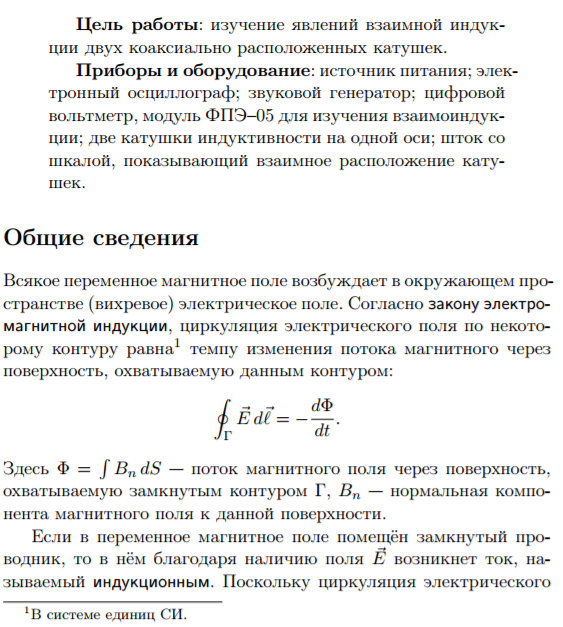
\includegraphics[width=15cm]{theory1.png}
    	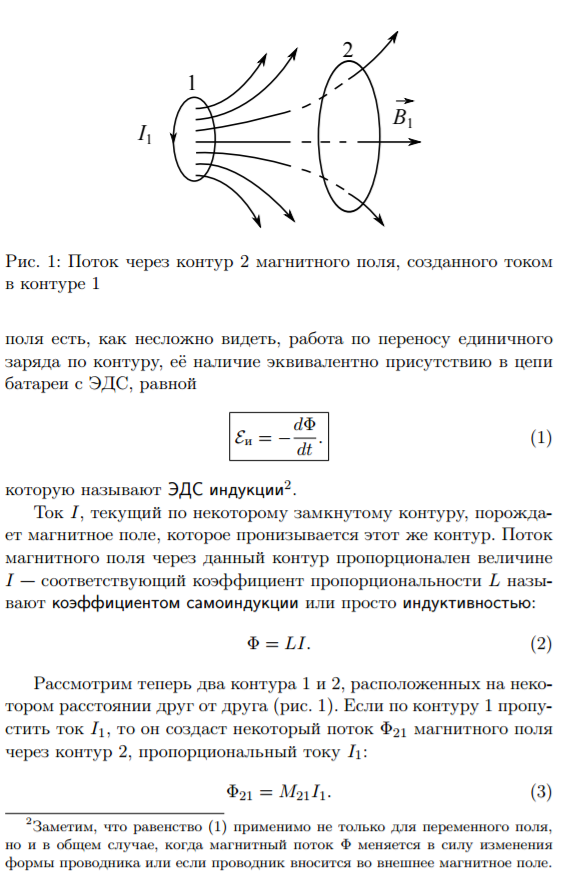
\includegraphics[width=15cm]{theory2.png}
    	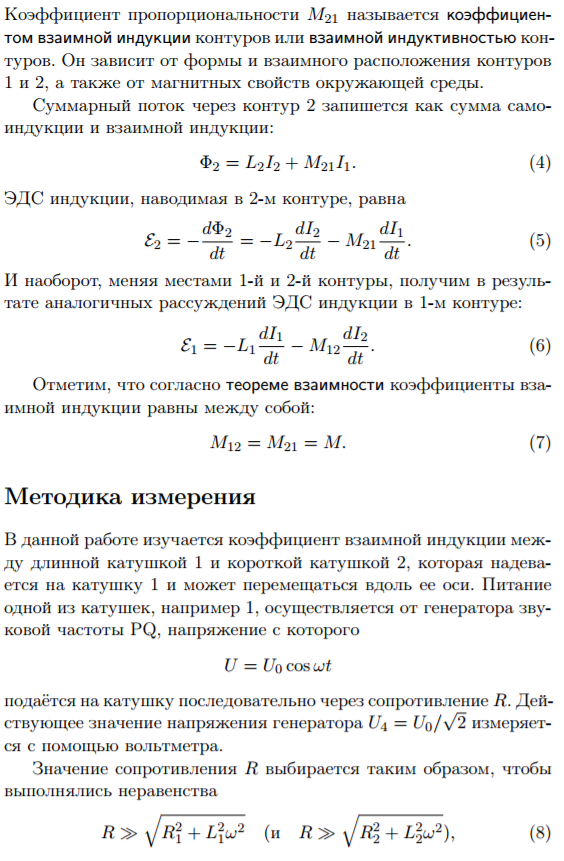
\includegraphics[width=15cm]{theory3.png}
    	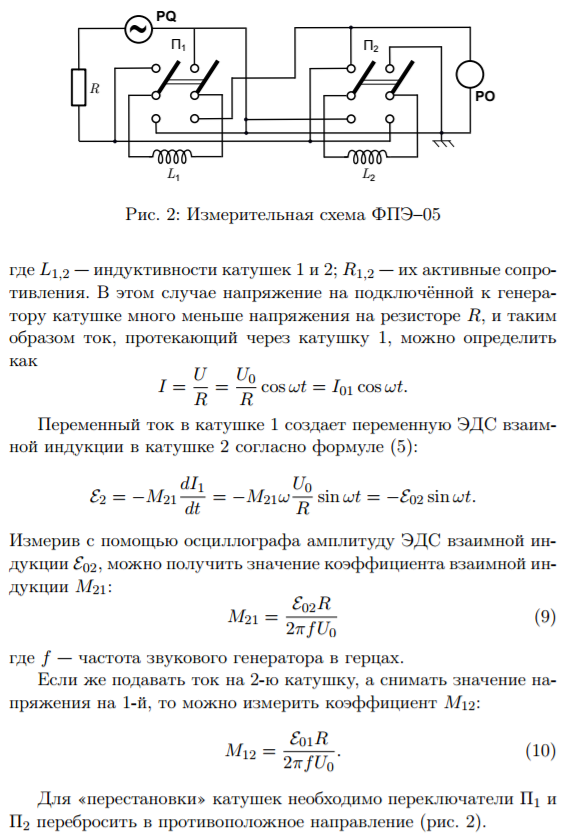
\includegraphics[width=15cm]{theory4.png}
    	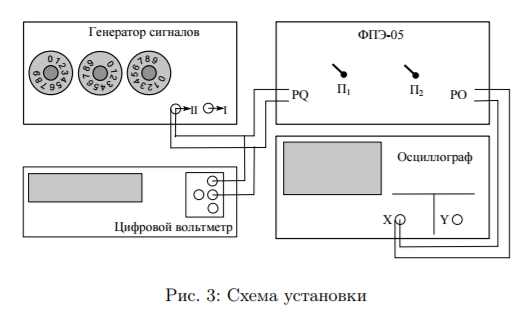
\includegraphics[width=15cm]{theory5.png}
    \end{center}
    
    \begin{center}
       	\textbf{\large{Выполнение работы}}
    \end{center}
    
    Соберём схему (рис. 3). Задав напряжение генератора $U_4 = 3B$ Подключив к установне сначала первую, затем вторую катушку, проверим, что в рабочем диапазоне частот (5 - 25 кГц) $\mathcal{E}_{0i} / f = const$, т. е. амплитуда напряжения на катушке линейно зависит от частоты.
    
    \begin{center}
    	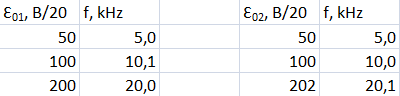
\includegraphics[width=10cm]{table1.png}
    \end{center}
    
    Как видим, зависимость действительно линейная.\\\\
    
    Для измерения коэффициента взаимной индукции М21 установим переключатель П1 в положение PQ, а переключатель П2 в положение PO. При этом напряжение звукового генератора подаётся на катушку 1, а ЭДС с катушки 2 подаётся на вход осциллографа. Теперь будем постепенно выдвигать катушку 1 и замерим зависимость $\mathcal{E}_{02}(z)$, где z - на сколько выдвинута катушка. При измерениях $U_4=3B$, $f=15kHz$. $R = 10,5 \pm 0,5 kOm$. M21 будем искать по формуле (9).
    
    Аналагично измерим M12(z).
    
    \begin{center}
    	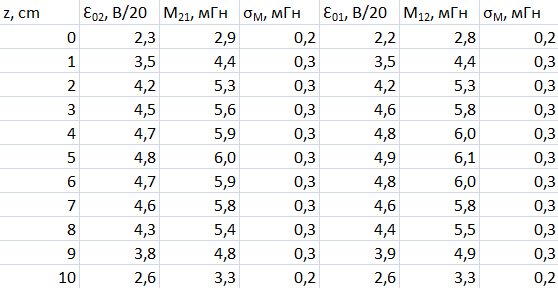
\includegraphics[width=14cm]{table2.png}
    \end{center}
    
    Как видим, в пределах погрешности $M_{12} = M_{21}$. Т. е. выполняется теорема взаимности.
    
    Построим график М(z):
    
    \begin{center}
    	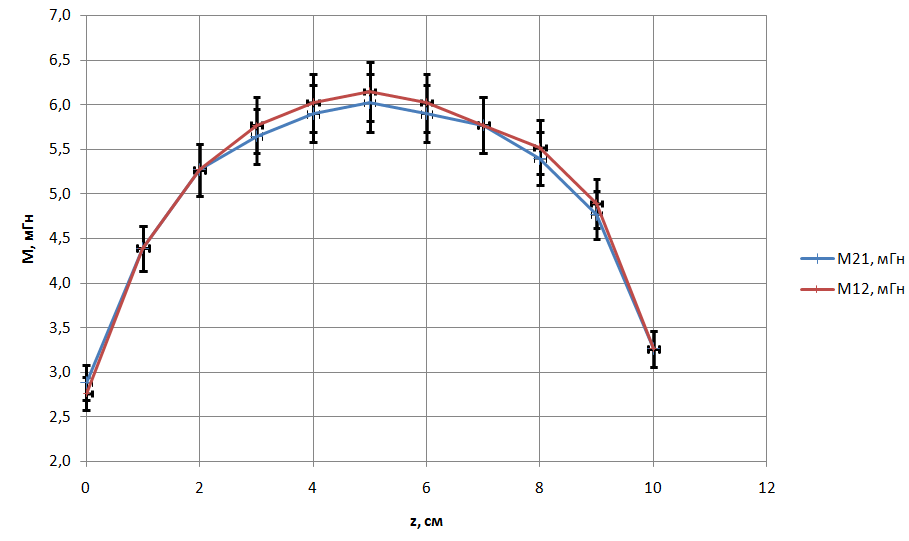
\includegraphics[width=17cm]{graph1.png}
    \end{center}
    
    Теперь убедимся в том, что коэффициент взаимной индукции не зависит от напряжения на генераторе.
    
    Для этого выдвинем катушку на z=5cm, установим f=15kHz. Измерим $\mathcal{E}_{02}$ при нескольких значениях $U_4$:
    
    \begin{center}
    	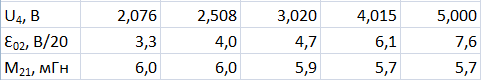
\includegraphics[width=10cm]{table3.png}
    \end{center}
    
    Погрешность вычисленных $M_{21}$ точно не меньше 5\% (именно такая погрешность у сопротивления R), значит абсолютная погрешность не меньше 0,3мГн. Мы видим, что с учётом погрешности коэффициент взаимной индукции не зависит от входного напряжения.\\ \\
    
    Теперь определим эксперементально зависимость коэффициента взаимной индукции от частоты генератора.
    
    Установим z=5cm, $U_4 = 3B$. Измерим $\mathcal{E}_{02}$ при нескольких значениях $f$:
    
    \begin{center}
    	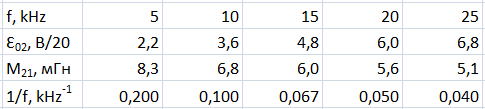
\includegraphics[width=12cm]{table4.png}
    \end{center}
    
    Как видим, зависимость $M_{21}(\frac{1}{f})$ линейная.
    
    \begin{center}
    	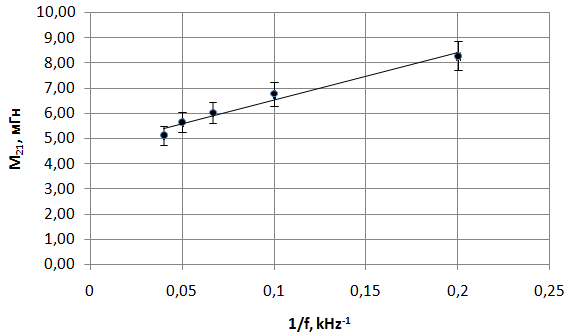
\includegraphics[width=12cm]{graph2.png}
    \end{center}
    
    Погрешность M(f) около 5\%, ибо в формуле (9) наибольшая погрешность R как раз 5\%.
    
\end{document}